\documentclass[portrait, A0]{sciposter}
\usepackage{ebgaramond}
\setsansfont{EB Garamond}
\usepackage{fontspec}

\usepackage{lipsum}
\usepackage{epsfig}
\usepackage{amsmath}
\usepackage{amssymb}
\usepackage{graphicx,url}
\usepackage{tikz}

\usepackage{multicol}
\setlength\columnsep{19pt}
\usepackage{siunitx}
\sisetup{
    detect-all,
    output-decimal-marker={,},
    group-minimum-digits = 3,
    group-separator={~},
    number-unit-separator={~},
    inter-unit-product={~}
}
% Tableau
\usepackage{array,multirow,makecell}
\setcellgapes{1pt}
\makegapedcells

% Réglages fins
\setlength{\parindent}{2em}
\usepackage{caption}
\captionsetup{font = footnotesize, labelsep = period}
\usepackage{paracol}
%Hyper lien
\usepackage{hyperref}

%% Réglages -- Notes de BdP
%\usepackage[para]{footnotes}
\renewcommand*\footnoterule{}
\setlength{\footnotesep}{0.5cm}

%%% Figures

\usepackage{graphicx}
%\usepackage{subcaption}

\usepackage{blindtext}
\usepackage[inline]{enumitem}

\usepackage[english, french]{babel}
\usepackage[french=guillemets]{csquotes}

% Personnalisations diverses 
\addto\captionsfrench{\renewcommand{\figurename}{\textsc{Map}}}

% Ecrire les unités  edmesur 
\usepackage{siunitx}

%------------------------------------------------			
% Guillemets corrects, commande G
\usepackage{xspace}

\title{Index toponymique de la Planche 52}

\institute{EHESS}

\rightlogo[1]{gfx/village.pdf}
\leftlogo[1]{}

%%%%%%%% Préambule - f
%\usepackage[showframe]{geometry}

%%%%%%%% Crop

\usepackage[a0,frame,axes,cross,pdftex,center]{crop}
\usepackage{layout}
%\usepackage{showframe}

\begin{document}
\conference{\bf Index toponymique de la Planche 52 - épreuves V1 (\today) - à corriger}
\bgroup
\setlength{\parindent}{-0.1em} 
\begin{minipage}[t]{0.6\textwidth}
  \Huge
  \textsc{Engraved Footprints from the Past}\\ \\
  \Large \textsc{Retrieving Cartographic Geo-Historical Data from Cassini’s \emph{Carte de France}, 1750 - 1789}
\end{minipage}
\begin{minipage}[t]{0.35\textwidth}
  \vspace*{-2.5cm}
  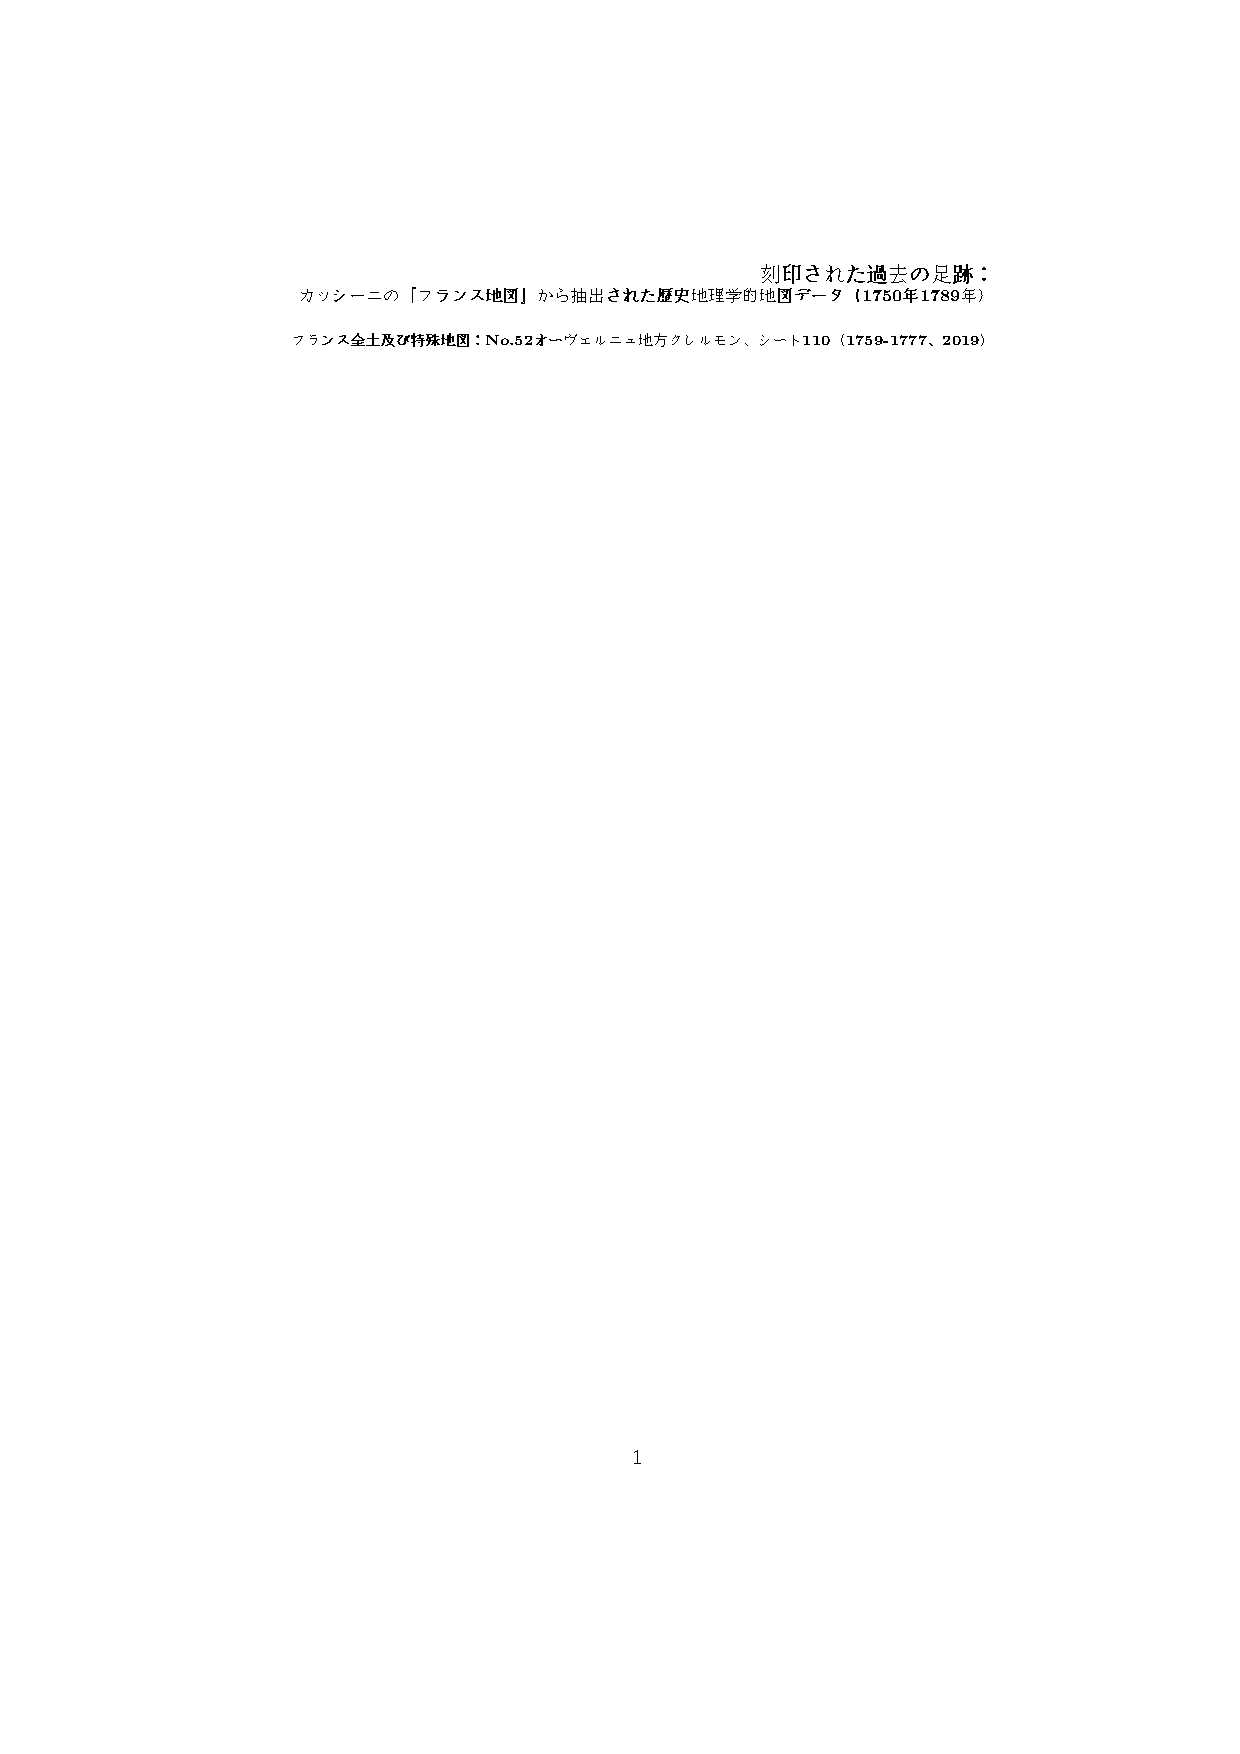
\includegraphics[width=\textwidth, trim= 5cm 26cm 4cm 22cm, clip]{gfx/jap.pdf}
\end{minipage}

\vspace{1cm}
\egroup

\begin{minipage}[b]{75cm}
%%% Begin of Multicols-E
%\setlength{\columnsep}{40pt}
\begin{multicols}{3}
\setlength{\columnsep}{80pt}
%\section{0}

%\section{Abstract}
\section*{\normalfont B. \textsc{Duménieu}, J. \textsc{Chadeyron}, P. \textsc{Cristofoli}, J. \textsc{Perret} and S. \textsc{Baciocchi}, in collaboration with S. Gomis, M. Gribaudi, I. Langlois, C. Motte and M.-C. Vouloir}
\lettrine{A}ntique maps are full of engraved geo-historical features. They provide past representations of the geographical space, favored by historians and social scientists for their uniqueness and coherence. Working on a GIS dedicated to the history of French territory, we extracted spatial information from Cassini’s \textit{Carte de France} as vector data. Based on the first geodetic survey of France [1, 4], this well-known map has been drawn on 182 paper sheets of size 610 x 955~mm at the scale of 1:86~400 or 1 line for 100~toises (\textit{i.e.} 1 inch to 1.36 miles). It depicts the French territory with fine-grained information about populated and named places, settlements, landscape features, hydrographic, ecclesiastical and road networks [3, 5, 6, 7]. As a case study, the sheet numbered 52 provided more than 6,800 spatial footprints that we have stored as a geographical database. Following the distinction made by Cassini himself between \og geometric \fg and \og topographic \fg entities, our geographical database is composed of two kinds of data, namely 1) Triangulated Geographical Entities (\og geometric \fg entities in Cassini’s own terms) whose geodetic properties are partly documented and 2) Relative Geographical Entities (\og topographic \fg in Cassini’s terms) which are dependent on and located relative to the former (Map. \ref{map:triangulated-relative}). Those entities are analytically distinct but come together from a same and single artifact, \emph{i.e.} the primary source they have been engraved in during the mapmaking process (Map. \ref{map:contours}). Because this process of embeddedness is not fully documented, retrieving both classes of entities called for a cautious cartographic visualization with similar semiological rules and aesthetics as the original historical map. This \og Cassini's Mapping Style \fg allows to keep the cartographic properties of the geo-historical data extracted from this primary source: generalisation, scale, spatial granularity and the overall intentions of the mapmakers [2]. Often neglected, such properties are constitutive components and dimensions of the mapping style which forms the context and gives crucial information on the accuracy and the relationships between geo-historical data enclosed in. Our GIS-based map (Map. \ref{GIS-based map}),  which comes with its own legend and some statistics (Tab. \ref{tab:stats} and \ref{tab:symbols}), provides a renewed cartographic visualization of the entire sheet 52. It reveals unnoticed cartographic entities that were hardly legible in the original map (Fig. 4a-b).\\
\vfill


\small
\textbf{[1]} C.-F. Cassini (1783). \textit{Description géométrique de la France}. Imprimerie Desaint.
[2] S. Christophe, B. Duménieu, A. Masse, C. Hoarau, J. Ory, M. Brédif, F. Lecordix, N. Mellado, J. Turbet, H. Loi, T. Hurtut, D. Vanderhaeghe, R. Vergne, and J. Thollot. Expressive map design: Ogc sld/se++ extension for expressive map styles. \textit{Proceedings of the ICA}, 1:21, 2018.
[3] F. de Dainville. La carte de Cassini et son intérêt géographique. \textit{Bulletin de l'Association des géographes français}, 32(251), 138-147, 1955.
[4] J. V. Konvitz. Redating and rethinking the cassini geodetic surveys of france, 1730–750. \textit{Cartographica : The International Journal for Geographic Information and Geovisualization}, 19(1) :1–15, 1982.
[5] C. Motte and M-C. Vouloir. Le site \href{http://cassini.ehess.fr}{Cassini.ehess.fr}: un instrument d’observation pour une analyse du peuplement. \textit{Revue du Comité Français de Cartographie}, 191, 68–84, 2007.
[6] J. Perret, M. Gribaudi, M. Barthelemy, N. Abadie, S. Baciocchi, C. Bertelli, O. Bonin, P. Bordin, B. Costes, P. Cristofoli, B. Duménieu, J. Gravier, J.-P. Hubert, P.-A. Le Ny, E. Mermet, C. Motte, M. Pardoen, A.-M. Raimond, S. Robert, and M.-C. Vouloir. The 18\up{th} century Cassini roads and cities dataset, \textit{Harvard Dataverse}, 2015.
[7] J. Perret, M. Gribaudi, and M. Barthelemy. Roads and cities of 18\up{th} century france. \textit{Scientific data}, 2 :150048, 2015.

%\switchcolumn
\begin{center}
 \captionof{figure}{\scriptsize{Triangulated and Relative Geographical Entities \\in the 52\up{nd} sheet of the Cassini map (1759-1777)}}
 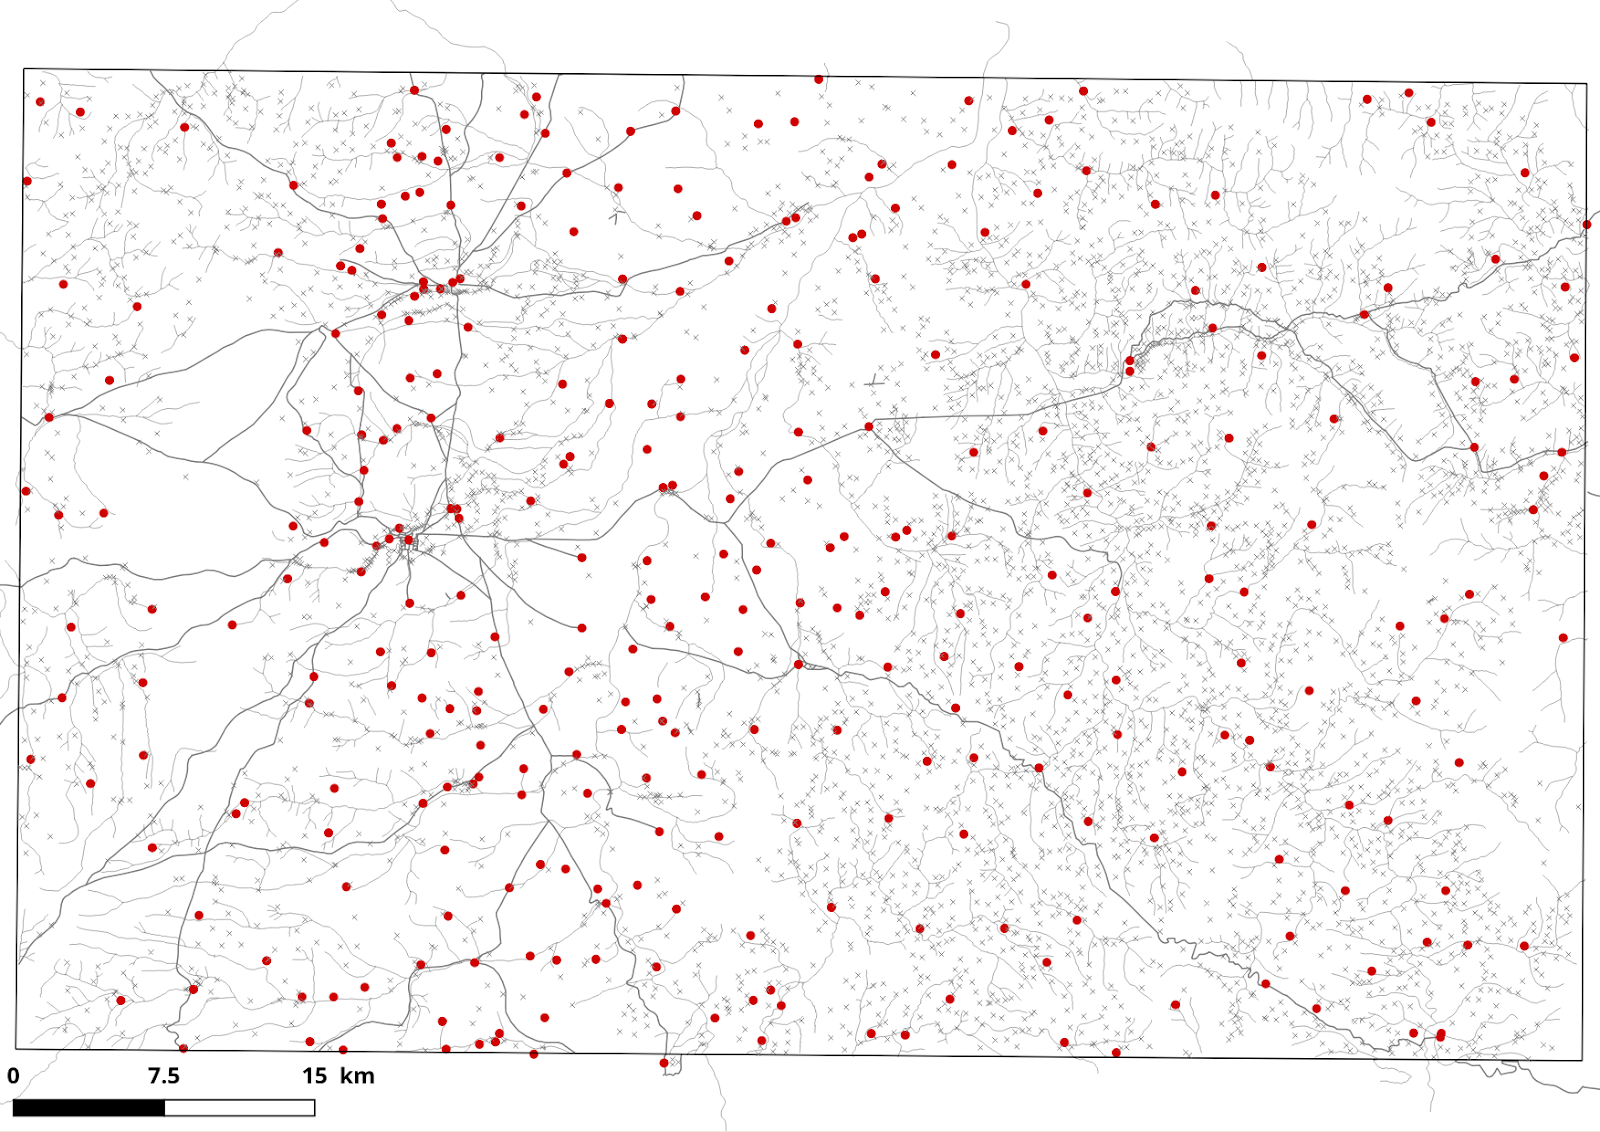
\includegraphics[width=21cm]{gfx/Triangulated.png}
 \label{map:triangulated-relative}
 \vfill
  Analytical map of all the geographical features surveyed,\\ whether triangulated (k=316 in red) or relative (n=6,565 in grey).
 \end{center}
 
\end{multicols}
\end{minipage}
%%%%

\begin{minipage}[b]{75cm}
  \section{\normalfont \textsc{Digital reconstruction of \og Carte générale \textsc{\textit{\&}} particulière de la France \fg } with a  \og Cassini \fg map style (2019)}
\begin{center}
\captionof{figure}{GIS-based cartographic visualization of the \og Carte générale \textsc{\textit{\&}} particulière de la France \fg, \textsc{n}\up{o} 52 Clermont en Auvergne. F\up{le} 110: 1759-1777\protect\footnotemark}
  \footnotetext{\up{1}. The original historical map has been geo-referenced, vectorized and digitally rendered at a decreased scale of 1: xx~xxx under QGIS and \LaTeX ~by the team \textsc{GeoHistoricalData} (EHESS / IGN / UCA) in 2016-2018: Nathalie \textsc{Abadie}, Stéphane \textsc{Baciocchi}, Pierre \textsc{Boivin}, Julien \textsc{Chadeyron}, Pascal \textsc{Cristofoli}, Jean-Michel \textsc{Delaveau}, Bertrand \textsc{Duménieu}, Stéphane \textsc{Gomis}, Maurizio \textsc{Gribaudi}, Isabelle \textsc{Langlois}, Claude \textsc{Motte}, Julien \textsc{Perret} \textsc{\textit{\&}} Marie-Christine \textsc{Vouloir}. Printed in Saint-Mandé in January 2019 by Thierry \textsc{Chaffaud} and Régis \textsc{Fiol} in the IGN Printed Products Manufacturing Department. With the support of the Centre de Recherches Historiques (EHESS/CNRS), the Centre d'Histoire \og Espaces \& Cultures \fg (UCA), the Laboratoire des Sciences et Technologies de l'Information Géographique - LaSTIG (IGN), the Laboratoire de Démographie et d'Histoire Sociale (EHESS - Centre d) recherch eehistori uqsesand the SoDUCo project (ANR).}
 \includegraphics[width=75cm]{gfx/cassini_52_lr.pdf}
 \label{GIS-based map}
 \vfill
 \end{center}
\end{minipage}

 \begin{tikzpicture}[remember picture, overlay]
      \node[anchor=north west] at (0,7.5){%
        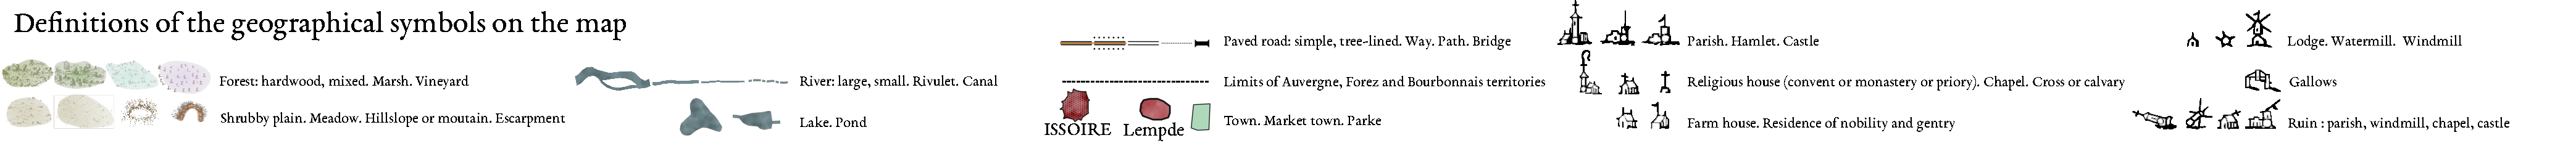
\includegraphics[width=61cm]{gfx/maplegend.pdf}};
\end{tikzpicture}

\begin{minipage}[b]{75cm}
\section{\normalfont \textsc{Retrieved geo-historical features}: some statistics}
\begin{multicols}{3}
\setlength{\columnsep}{80pt}

%\tiny{a variety of symbols mark smaller settlements: churches, wind and water mills, gallows and other works of man. Residences of nobility or gentry.

%\og
%The divided horizontal semi-circles in brass were fitted with telescopic alidades, and micrometer reading allowed angles to be observed with considerable accuracy.
%Beacons, and sometimes lights, were used for observation marks.
%The topographic detail was treated more summarily: though the plane table was commonly in use by the 'ingenieur géographes', the body of military surveyors, Cassini's men who carried out the minor triangulation sketched the details by estimation or by pacing, and worked this up in the office.
%Often they were content to indicate slopes by the letters D or F ('douce' or 'forte')
%\fg [Crone 1953:131]
%}
%bs%eclitartion{Triangulation \& projection}
%\subsection{Julien}
\footnotesize
\captionof{table}{Distribution of areas by land use type in the 52\up{nd} sheet of the Cassini map (1759-1777)}\label{tab:stats}

\setcellgapes{2pt}

\begin{tabular}{l|cccccccc|c|ccccc|c|r}

& \multicolumn{8}{c|}{Landscape feature}
& 
& \multicolumn{5}{c|}{Hydrography}
&
&\\
&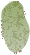
\includegraphics[height=40pt]{gfx/foret_couleur.png}
&
\includegraphics[height=40pt]{gfx/marais_couleur.png}
&
\includegraphics[height=40pt]{gfx/vigne_couleur.png}
&
\includegraphics[height=40pt]{gfx/landes_couleur.png}
&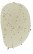
\includegraphics[height=40pt]{gfx/broussailles_couleur.png}
& 
\includegraphics[height=30pt]{gfx/domaine_couleur.png}
&
\includegraphics[height=35pt]{gfx/escarpement_couleur.png}
& \rotatebox{90} {\tiny{Farmland}}
&
\includegraphics[height=35pt]{gfx/ville_couleur.png}
&
\includegraphics[height=25pt]{gfx/etang_couleur.png}
&
\includegraphics[height=35pt]{gfx/riviere_large_couleur.png}
&
\includegraphics[height=30pt]{gfx/lac_couleur.png}
&
\includegraphics[height=30pt]{gfx/riviere_medium_couleur.png}
&
\includegraphics[height=30pt]{gfx/riviere_small_couleur.png}
&
\includegraphics[height=30pt]{gfx/routes_couleur.png}
&\textsc{Total}\\
Features count&257&32&111&-&150&6&-&-&37&240&-&9&-&-&-&-\\
Area sum (km\up{2})&\num{279}&\num{75}&\num{87}&\num{1368}&\num{142}&\num{0,6}&\num{0,8}&\num{1871}&\num{4}&\num{4}&\num{19}&\num{1,2}&-&-&-&\num{3852} km\up{2}\\
\makecell[r]{\textit{\% Map area}}&\textit{7}&\textit{2}&\textit{2}&\textit{36}&\textit{4}&\textit{0}&\textit{0}&\textit{49}&\textit{0}&\textit{0}&\textit{0}&\textit{0}&&&&\textit{100 \%}\\
Linear lenght (km)&-&-&-&-&-&-&-&-&-&-&-&-&\num{341}&\num{2841}&\num{624}&\num{3807} km
\end{tabular}

%\subsection{Pascal}

%\subsection{Pascal}
%\begin{center}
\footnotesize

\captionof{table}{Map symbols census in the 52\up{nd} sheet of the Cassini map (1759-1777)}\label{tab:symbols}
%\vspace{0.25cm}
\setcellgapes{2pt}
\begin{tabular}{cccccccccccccccc}
 %  \hline
% & & & & & & & & & & & & &//
%\textsc{  Caractères géographiques   }&
%\rotatebox{90} {\textsc{Total}} &
%\rotatebox{90} {Villes} &
%\rotatebox{90} {Bourgs} &
%\rotatebox{90} {Clochers} &
%\rotatebox{90} {Abbayes} &
%\rotatebox{90} {Prieurés} &
%\rotatebox{90} {Chapelles}&
%\rotatebox{90} {Calvaires}&
%\rotatebox{90} {Châteaux} &
%\rotatebox{90} {Hameaux}  &
%\rotatebox{90} {Gentillomières} &
%\rotatebox{90} {Maisons} &
%\rotatebox{90} {Moulins à eau} &
%\rotatebox{90} {Moulins à vent} &
%\rotatebox{90} {Justice} &
%\rotatebox{90} {Autres lieux} \\
&

\includegraphics[height=28pt]{gfx/ville_couleur.png}&
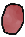
\includegraphics[height=25pt]{gfx/bourg_couleur.png}&

\includegraphics[height=40pt]{gfx/village.pdf}&
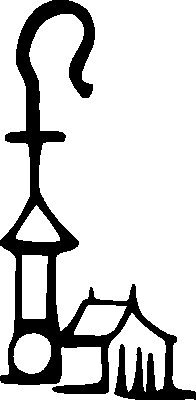
\includegraphics[height=49pt]{gfx/abbaye.pdf}&
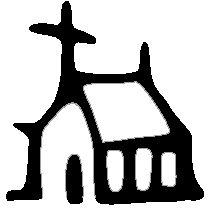
\includegraphics[height=30pt]{gfx/chapelle.pdf}&
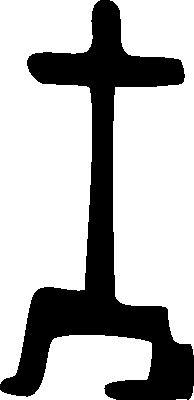
\includegraphics[height=30pt]{gfx/cross.pdf}&

\includegraphics[height=45pt]{gfx/chateau.pdf} &
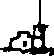
\includegraphics[height=40pt]{gfx/hameau.pdf}&
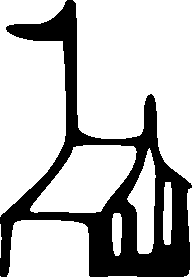
\includegraphics[height=35pt]{gfx/gentilhommiere.pdf}&
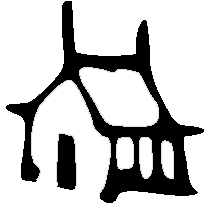
\includegraphics[height=30pt]{gfx/maison.pdf}&
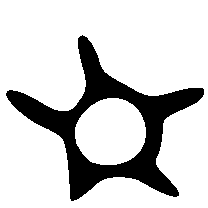
\includegraphics[height=30pt]{gfx/moulin_a_eau.pdf}&

\includegraphics[height=35pt]{gfx/moulin_a_vent.pdf}&
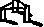
\includegraphics[height=18pt]{gfx/justice.pdf}&
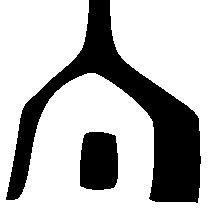
\includegraphics[height=18pt]{gfx/cabane.pdf}&
\rotatebox{90}{\textsc{Total}}\\
% \multicolumn{14}{|c|}{} \\
% \hline
\makecell[l]{Symbols count} & \num{15} & \num{22} & \num{234} & \num{11} & \num{93} & \num{28} & \num{196} & \num{2277} & \num{39} & \num{1135} & \num{501} & \num{1} & \num{5} & \num{6} & \num{4563}\\
\makecell[r]{\textit{of which unnamed}} & \textit{-} & \textit{-} & \textit{1} & \textit{2} & \textit{25} & \textit{15} & \textit{46} & \textit{28} & \textit{1} & \textit{52} & \textit{427} & \textit{-} & \textit{4} & \textit{1} & \textit{\num{601}}\\
 & & & & & & & & & & & & & & & \\
% \hline
% \makecell[c]{\textsc{Avec toponymes}} &  &  &  &  &  &  &  &  & &  & &  &  &  & \\
% \makecell[c]{\textsc{Sans toponyme}} &  &  &  &  &  &  &  &  &  & & &  &  &  & \\
% \hline
%\caption{nom du tableau}
%\multicolumn{14}{|c|}{} \\
\end{tabular}

%\end{center} 
%\subsection{Stephane, Bertrand}

%\subsection{Pascal}


\end{multicols}
\end{minipage}

\begin{minipage}[b]{75cm}
\section{\normalfont \textsc{Primary sources, mapmaking process \textit{\&} final result}}

\begin{multicols}{3}
\setlength{\columnsep}{80pt}

\textsc{Toward a critical edition} \small{of the...}
\vfill
\normalsize
\lettrine{O}riginal 610 x 955~mm colour map (format \og grand aigle \fg) on a scale of 1: 86~400 or 1 line for 100 toises. Drawn up from 1759 to 1777 under the direction of César François \textsc{Cassini de Thury}, Charles Étienne Louis \textsc{Camus} (then Rodolphe \textsc{Perronet}) and Étienne \textsc{Mignot de Montigny}. \textbf{Triangulated from 1759 to 1775} by P.~de~\textsc{La~Court} (\textsc{ne} partial, 1759), François \textsc{Pasumot}, Claude \textsc{Pezet}, \textsc{Dallier} and \textsc{Dailley} (\textsc{no-so}, c. 1764-1766), Louis \textsc{Le~Bel} (\textsc{se}, 1766-1768; \textsc{ne} and \textsc{so}, 1769), \textsc{Dubois} \textit{\&} Louis \textsc{Cabay} (\textsc{no-ne}, 1772-1773), Q\textsc{uerry} \textit{\&} François \textsc{La~Ruelle} (\textsc{ne}, 1774-1775). \textbf{Field checked, 1767-1774} by P. \textsc{Renault} (\textsc{se}, 1767-1768), Q\textsc{uerry} \textit{\&} F.~\textsc{La~Ruelle} (\textsc{no-ne-so}, 1774). \textbf{Map engraved in Paris in 1774-1777} by Louis \textsc{Capitaine} son (for the plan, 1774-1776) and Nicolas \textsc{Bourgoin} (for the letter, 1775-1777). Printed intaglio on the press of Paris Observatory in 1777 on behalf of the Compagnie associée pour la Carte générale de la France. Presented to the King and the Royal Court, Versailles, April 16, 1777 (\og silk printing \fg).\\
\vfill


\scriptsize Main primary sources: \textsc{BnF} (Paris) - Cartes et plans, GE C-22286 (Rés), \textit{Nouvelle carte qui comprend les principaux triangles qui servent de fondement à la description géométrique de la France, levée par ordre du Roy}, par mess. Maraldi et Cassini de Thury, 1744 ; Carthotèque de l'IGN (Saint-Mandé) - Minutes de la Carte Cassini (feuille 52) ; Registre < A > \textit{Registre des Ingénieurs et Vérificateurs, paraphé par nous, Directeurs de la carte de France}, le 15 juillet 1778, de Montigny, f.~94, 96 et 126 ; Registre  < E > -\textit{Copie du Journal de la Carte Générale de la France tenu par M\up{r}. [Jean-Charles] de Borda [, trésorier de la Société]}, commencé le 26 juin 1756 et fini le 1\up{er} juillet 1784.

\begin{center}
 \captionof{figure}{\scriptsize{Successive drafts of field surveys, map corrections and revisions, 1759-1775}}
 \label{map:contours}
 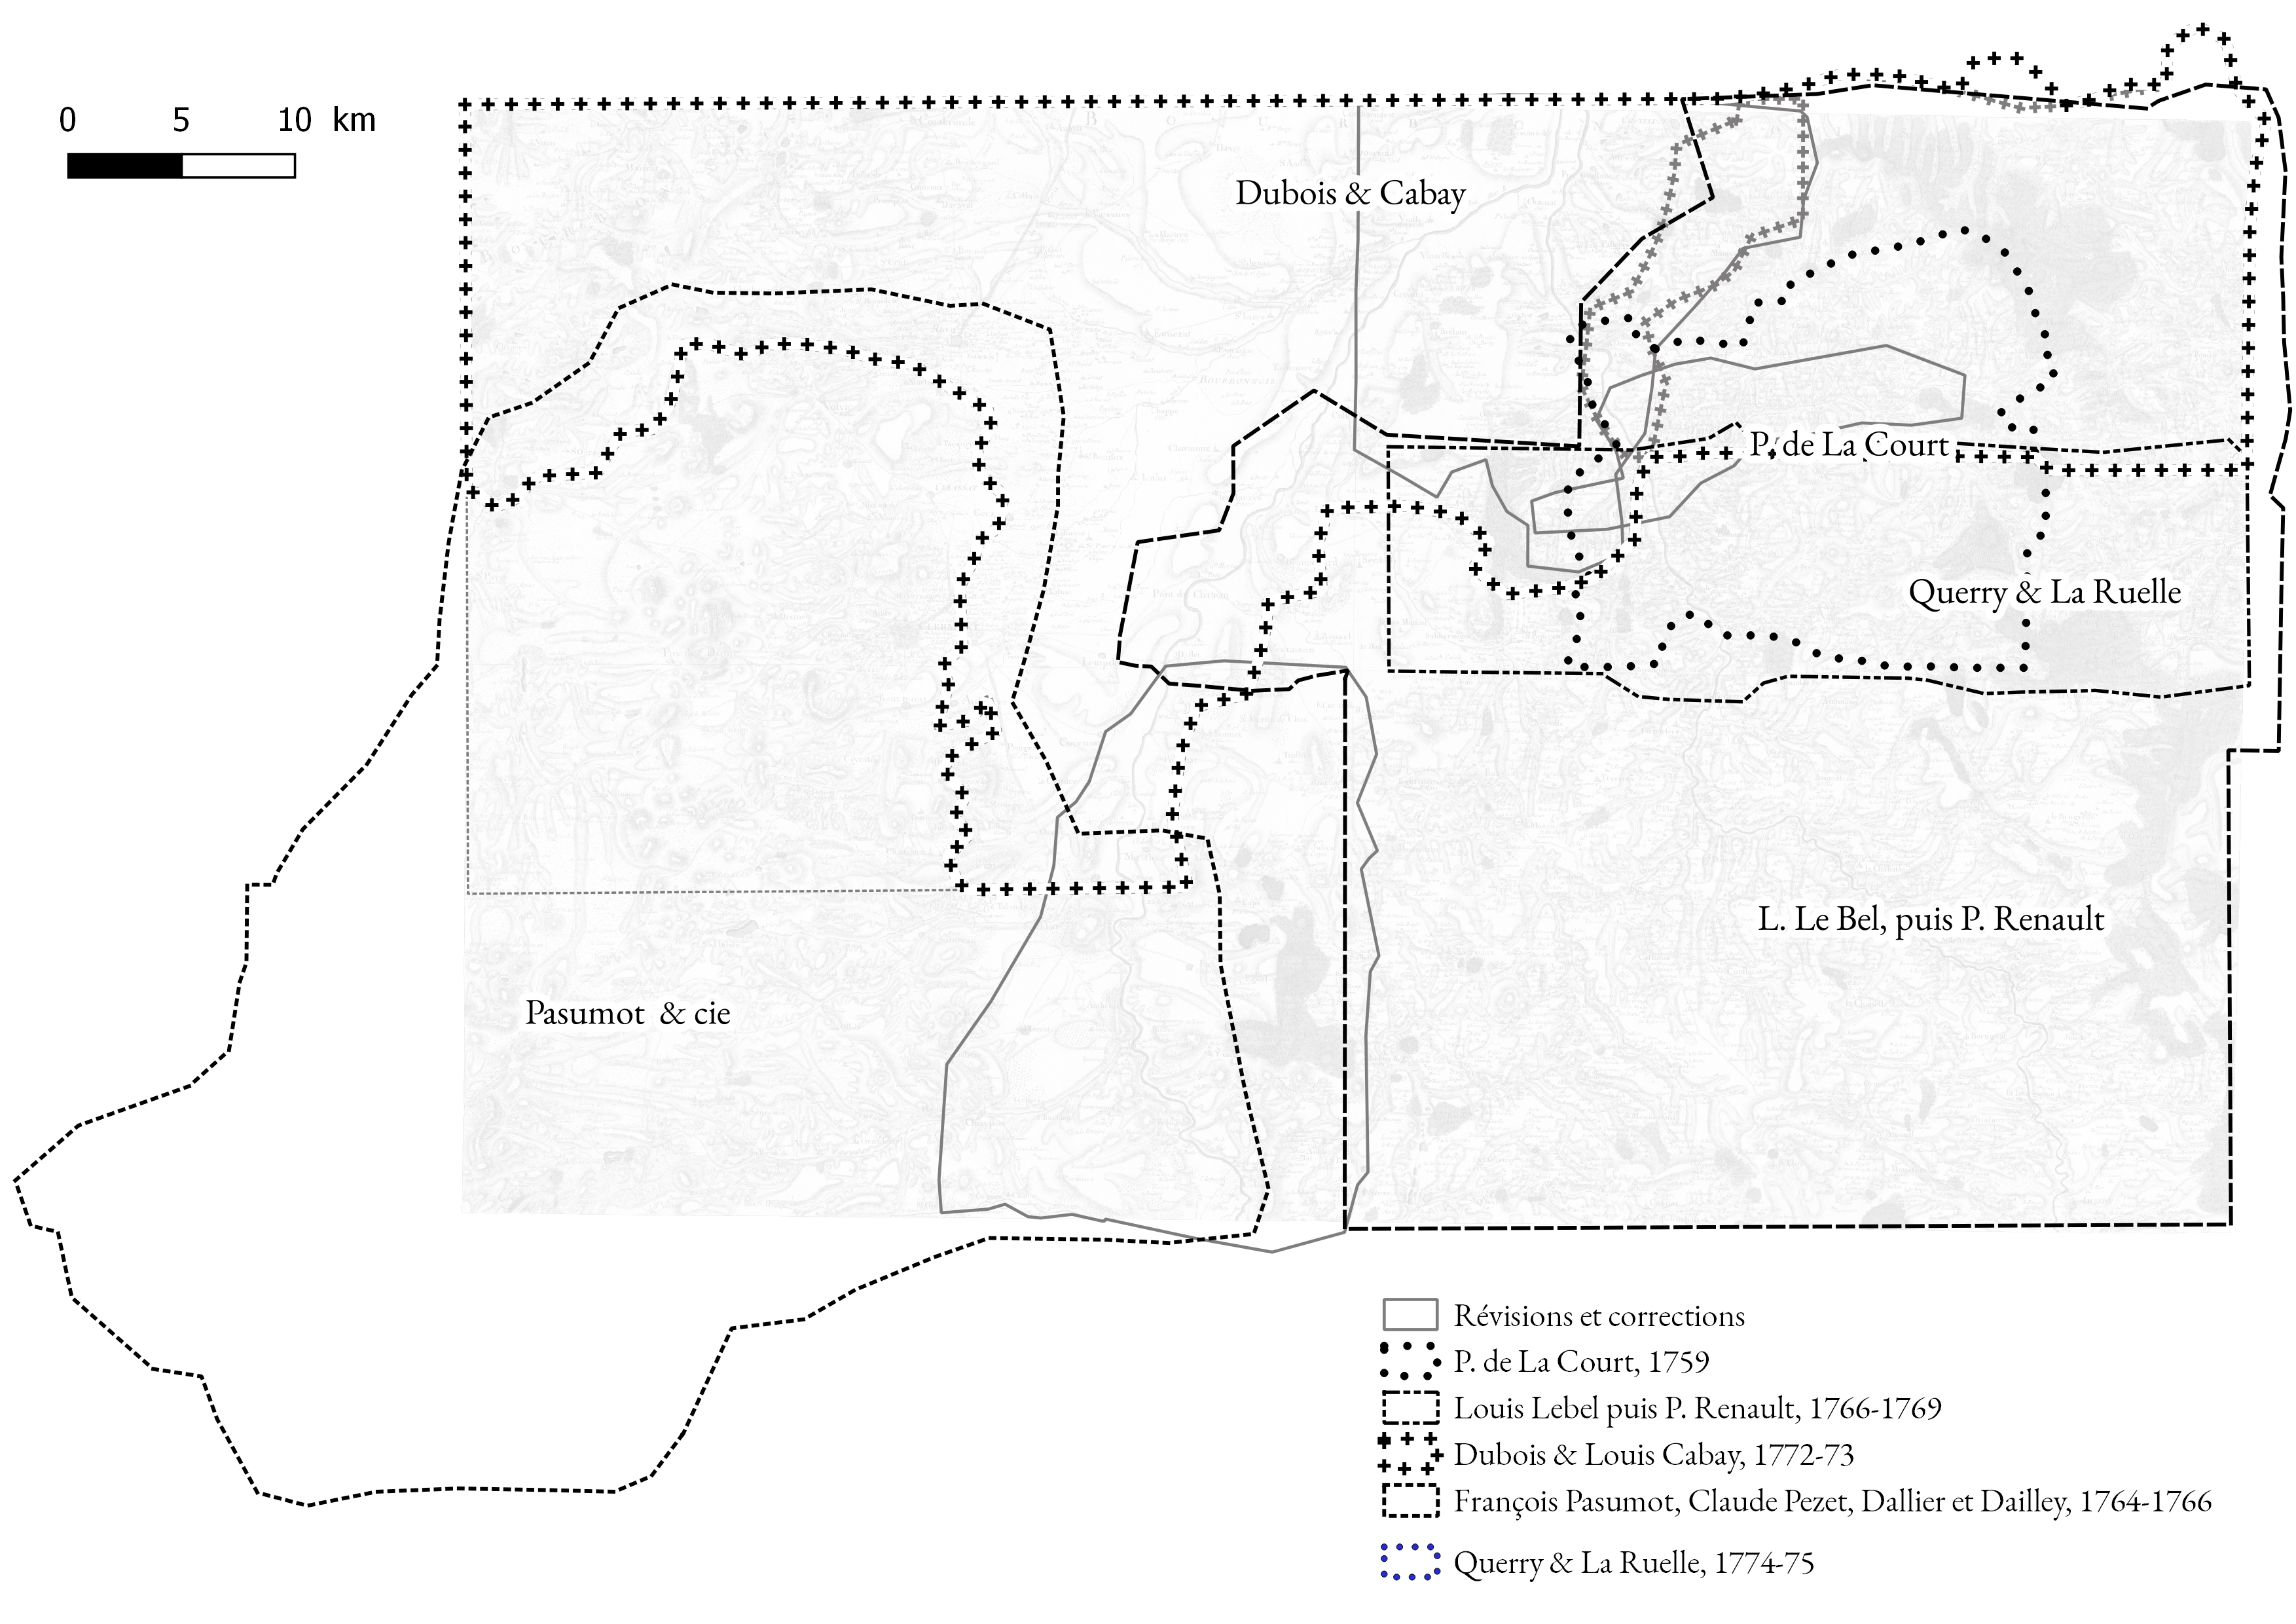
\includegraphics[width=21cm]{gfx/Contours.png}
 \end{center}

~\\
\normalsize
\textsc{From antique to renewed GIS-based hstorical map}


The history of cartography has been largely based on critical \emph{facsimile} edition of old maps. We propose to extend this approach by producing GIS-Based maps that combine the restitution of old styles and the geomatic modelling of geographical data.

\vfill

\begin{center}
 \captionof{figure}{\scriptsize{(a) a view on the original Cassini map of France (sheet 52, 1759-1777) and (b) the extracted vector data mapped with the \og Cassini \fg map style (2019)}}
 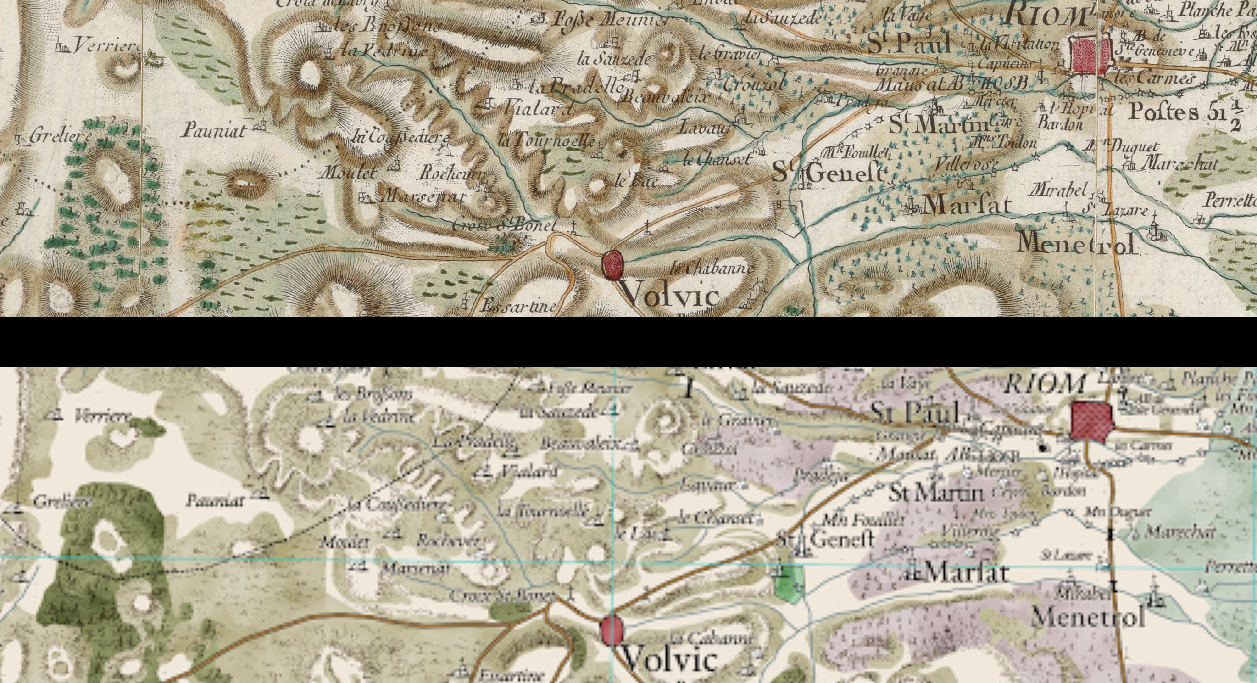
\includegraphics[width=21cm]{gfx/Fantome52extraits}
 \end{center}

%\scriptsize Proposition Pascal : établir la liste des couches QGis nécessaires à la construction de l'image issue de la base de donnée et les principaux problèmes liés à la conception (gérer les superpositions, la place des toponymes, le choix des couleurs, la généralisation de certains thèmes, etc...
\end{multicols}
\end{minipage}

\end{document}
